\subsection{Digitale Transformation mit Internet of Things}

Eine Umsetzung von Industrie-4.0-Lösungen setzt technische, organisatorische und normative Bedingungen voraus. Während einige Anforderungen für alle Bereiche in der Industrie gelten, unterscheiden sich explizite Anforderungen und Lösungen je nach individuellen Ausgangssituationen von Branchen und Unternehmen \citep{Bauer2014}. Dementsprechend werden im Folgenden zunächst allgemeine Anforderungen zur Umsetzung einer Lösung für die digitale Transformation näher beschrieben. Einen wesentlichen Stellenwert für die digtale Transformation hat das Cloud Computing als technische Voraussetzung, sodass es einer detaillierteren Erläuterung als in \ref{technologien} bedarf. Als Grundlage für die anwendungsfallbasierte Anforderungsanalyse in \ref{usecase} wird zuletzt ein Branchenbezug für die Energiewirtschaft hergestellt.

\subsubsection{Allgemeine Anforderungen zur Umsetzung von Industrie 4.0}

Im Rahmen der Industrie 4.0, die eine Spezialisierung des Internet der Dinge und Dienste darstellt, wachsen die virtuelle und reale Welt zusammen. Daraus ergibt sich die Herausforderung, die Anforderungen der IT, der Elektrotechnik sowie des Maschinenbaus miteinander zu vereinen \citep{Huebner2017}.

Aufgrund der heterogenen Landschaften und Aussgangssituationen der Unternehmen sei eine Standardisierung der Technologien laut \citet{Bauer2014} unerlässlich. Des weiteren ist die Weiterentwicklung von Breitbandnetzwerken für eine echtzeitfähige Kommunikation von Systemen eine Grundvoraussetzung. Notwendig sind außerdem qualitätsgesicherte Dienste im Internet, die robust gegen Störungen sind. Der Begriff \textit{Internet der Dinge und Dienste} bezieht auf vernetzte Komponenten wie physische Systeme, aber auch auf virtuelle Anwendungen. Da sich die Anzahl und die Beschaffenheit der Applikationen ebenso rasant ändern kann wie die der Geräte, ist eine standardisierte Laufzeitumgebung für diese von großer Bedeutung. Nicht zu vernachlässigen sind dabei die Sicherheitsaspekte. Die \ac{iot}-Anwendungen bilden eine große Angriffsfläche für Hacker, die durch Sabotage und Manipulation der Systeme eine große Gefahr dartellen. Ein historisches Beispiel für solch eine Gefahr sind die Stuxnet-Angriffe von 2010 auf iranische Atomfabriken \citep{Bauer2014}.

Allgmein können die Anforderungen und Voraussetzungen für eine \ac{iot}-Lösung auf folgende Begriffe projiziert werden \citep{Acharya2019}:

\begin{itemize}
  \item Skalierbarkeit und Flexibilität
  \item Schnelligkeit
  \item (Ausfall-)Sicherheit
  \item Qualität
\end{itemize}

Für speziellere Richtlinien enwickelte die Plattform Industrie 4.0 das \glqq Referenzarchitekturmodell Industrie 4.0\grqq{} (RAMI 4.0) sowie das Konzept der \glqq Industrie-4.0-Komponente\grqq{}.

\subsubsection{Standarrdisierung und Normung}

\begin{itemize}
  \item Bitkom bzw. Plattform Industrie 4.0 stellt Referenzarchitektur
  \item Industrie 4.0 ist eine Spezialisierung des Internet of Things and Services (Bitkom S.41)
  \item evtl. RAMI in Anforderungen in Part 3 packen mit angepasstem UseCase
  \item RAMI bietet die Möglichkeit, Industrie 4.0 UseCases zu verorten, um die für den jeweiligen use case notwendigen Normen und Standards zu identfizieren
  \item Schlagworte: Automatisierung, Sicherheit, Flexibilität, Wertschöpfungskette, Vernetzung
  \item Bitkom S. 16:
  \item horizontale Integration über Wertschöpfungsnetzwerke: Lieferanten, Unternehmen, Produzenten
  \item Durchgängigkeit des Engineerings: Systems Engineering, Modellierung, Simulation
  \item vertikale Integration und vernetzte Pproduktionssysteme mit Echtzeitanforderung
  \item neue soziale Infrastrukturen der Arbeit: Humane-Machine-Systeme und Usability
  \item kontinuierliche Entwicklung von Querschnittssystemen: Netzkommunikation, Breitband, Cloud, Data Analytics, Cyber security
\end{itemize}

(Industrie 4.0 Weltweit)

 Für die Bewältigung dieser Herausforderung veröffentlichte die Plattform Industrie 4.0 ein Referenzarchitekturmodell (RAMI 4.0) für die Industrie 4.0 als Grundlage für Standardisierung und Normung.

Das RAMI 4.0 basiert auf den Grundideen des Smart Grids, welches das Stromnetz von der Erzeugung bis zur Verteilung zum Endverbraucher behandelt. Das dreidimensionale Modell kapselt die wichtigsten Funktionalitäten in mehreren Schichten. Dies schafft Flexibilität für die Konzeptionisierung und Realisierung von Industrie 4.0-Lösungen.

\begin{itemize}
  \item Aspekte Industrie 4.0 (Bitkom S. 40) -> Für diese Ziele muss eine Referenz geschaffen werden
  \item 1 - vertikale Integration innerhalb der Fabrik/der Produktion: Vernetzung von Produktionsmitteln wie Automatisierungsgeräte oder Dienste untereinander
  \item 2 - Einbeziehung der Produktes (in meinem Fall produzierte Energie)
  \item durchgängiges Engineering bedeutet: technische, administrative, kommerzielle Daten rund um das Produktionsmittel über Wertschöpfungskette hinweg konsistent halten und jederzeit über das Netzwerk zugreifbar machen
  \item 3 - horizontale Integration über Wertschöpfungsnetzwerke über den Fabrikstandort hinaus und dynamische Bildung von Wertschöpfungsnetzwerken
  \item es gibt RAMI 4.0
  \item und Referenzmodell für die Industrie 4.0-Komponente (s. 45) mit Verwaltungsschale
\end{itemize}



Das Zusammenwachsen der pyhsischen und realen Welt zu mit Sensorik und Aktorik ausgestatteten Objekten, die mit dem Internet der Dinge miteinander vernetzt werden, erfordert eine Standardisierung \citep{BITKOM2015}.



Anforderung:Standardisierung


nach RAMI 4.0
RAMI (Referenzarchitekturmodell Industrie) 4.0: OPC-UA: Kommunikationsstandards (inkl. Sicherheit)
Sensorik: Bedeutung und sehr oberflächlich Funktionsweisen beschreiben
Gateways: Edge Processing
Device Management
Digital Twins

\begin{figure}[h]
  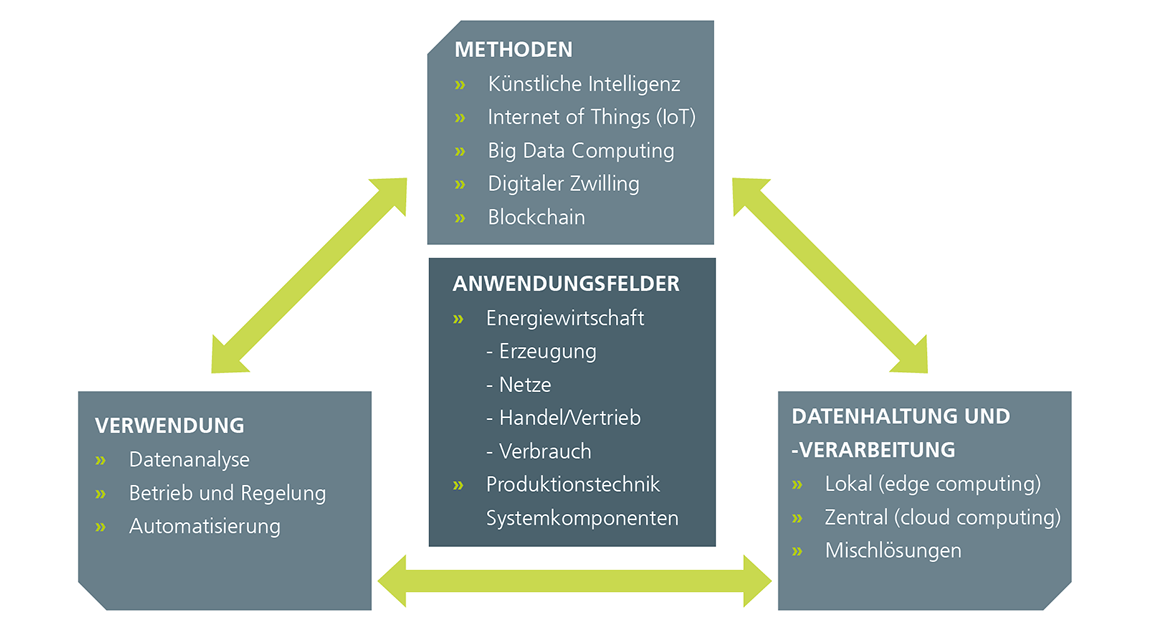
\includegraphics[width=1.0\linewidth]{dimensionen_digitalisierung_fraunhofer.png}
  \caption[Dimensionen der Digitalisierung]{Dimensionen der Digitalisierung \citep{FraunhoferISE}}
\end{figure}

% ************* CLOUD COMPUTING ******************
\subsubsection{Das neue Paradigma: Cloud Computing}

Für eine erfolgreiche digitale Transformation sind Geschwindigkeit, Flexibilität, eine hohe Qualität
sowie niedrige Kosten eine Grundbedingung \citep{Acharya2019}. Die Geschwindigkeit ist notwendig, um neue Funktionen zu veröffentlichen

Cloud-Native-Development -> neues Paradigma fernab vom 3-Thier Modell
IaaS, PaaS, SaaS, Microservices/SOA: service-oriented architecture
Integration modularer Services!= monolithische Strukur
Integration heterogener Datenquellen

\begin{quotation}
  cf push - and your app is alive
\end{quotation}


\subsubsection{Der Wandel im Energiesektor}
Welche Veränderungen durchlebt der Energiesektor?
Mechanisierung, Automatisierung und Digitalisierung sind die Schlagworte des industriellen Wandels, der auch die Energiewirtschaft betrifft.


Hier könnte man Bezug auf Energiesektor (kurz) nehmen und einführen, mit welchen Anforderungen und technologien generell so ein Wandel/Transformation stattfinden kann.
\begin{itemize}
  \item Disruption bestehender Geschäftsmodelle, vom Produzenten zum Dienstleister \citep{Doleski2017}
  \item dezentrale und fluktuierende Energieerzeugung erfordert digitale Lösungen
  \item wichtige Rolle kommunaler Unternehmen als Bereitsteller von Infrastrukturen wie Strom, Gas, Wärme, Wasser, Abwasser, Abfallwirtschaft, Stadtreinigung, Breitband \citep{Doleski2017}
  \item Beitrag zu funktionierendem Gemeinwesen, sozialer Teilhabe und Versorgungssicherheit -> Partner erster Wahl beim Gelingen der digitalen Transformation
  \item Wichtig für Gelingen: Erfahrungsaustausch, Kooperationen, richtige politische Rahmenbedingungen -> Katherine Reiche
  \item auf Unternehmensseite: Aufbau und Umsetzung einer unternehmensspezifischen Digitalisierungsstrategie: RAMI 4.0 als Referenz möglich
  \item Drei Revolutionen in der Energiewirtschaft \citep{Doleski2017}
  \begin{enumerate}
    \item Ab 1998: Liberalisierung und Privatisierung der Strommärkte fördert Wettbewerb, stellt aber eine Herausforderung Digitalisierungsstrategie
    \item Ab 2011: Energiewende und Aussteig aus Kernenergie fördert neue Technologien für erneuerbare Energien, aber die Berechenbarkeit der Kapazitäten verändert sich
    \item Digitalisierung: Potenzial für neue Revolution, Strom kann zwar nicht digitalisiert werden, aber die Vertriebsmodelle
  \end{enumerate}
  \item Datenschutz und Sicherheit gewinnen an Bedeutung
  \item Trend: Energieversorgungsunternehmen wandeln sich Richtung Dienstleitsungsunternehmen
  \item \glqq Mit der Zunahme dezentraler Einspeisungs- und Eigenversorgungsanlagen innerhalb der bestehenden Strom- und Gasnetze steigen synchron auch die Koordinationsanforderungen und die zu beherrschenden Datenmengen \grqq{} \citep[S. 7]{Doleski2016}
  \item \glqq Bedarf einer branchenweiten Veränderung - einer Transformation - in allen Sektoren und Phasen entlang der energiewirtschaftlichen Wertschöpfung\grqq{} \cite[S. 11]{Doleski2016}
  \item Utility 4.0: Digitale Enegergiedienstleistungsunternehmen
  \item Während nach Dampfmaschine, Massenproduktion und Automation nunmehr die Digitalisierung die vierte industrielle Revolution einläutet, unterliegt die Energiewirtschaft ähnlichen Entwicklungsprozessen.
\end{itemize}

\begin{figure}[h]
  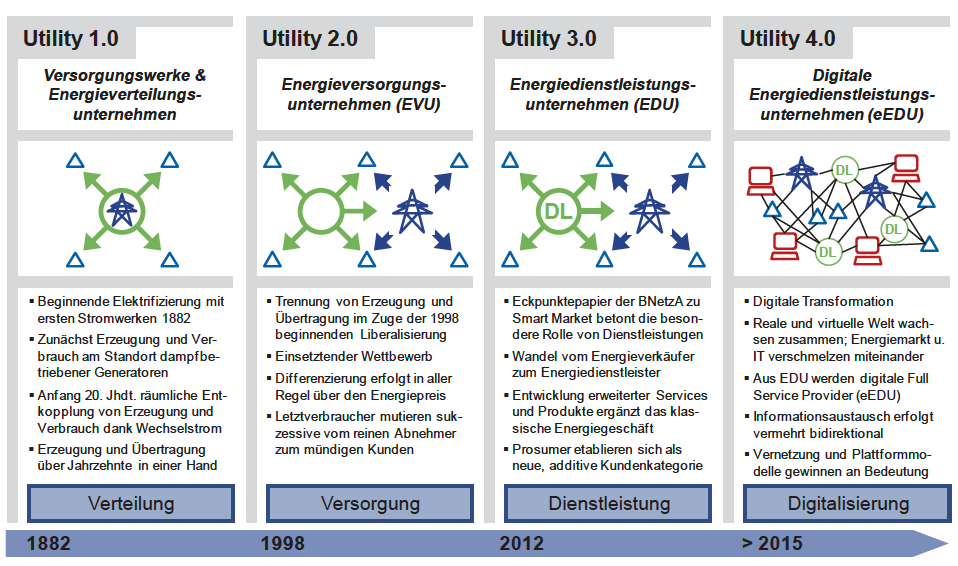
\includegraphics[width=1.0\linewidth]{utility_40.png}
  \caption[Transformation vom Versorgungswerk zum digitalen Energiedienstleister]{Transformation vom Versorgungswerk zum digitalen Energiedienstleister \citep[S. 13]{Doleski2016}}
\end{figure}

\begin{figure}[h]
  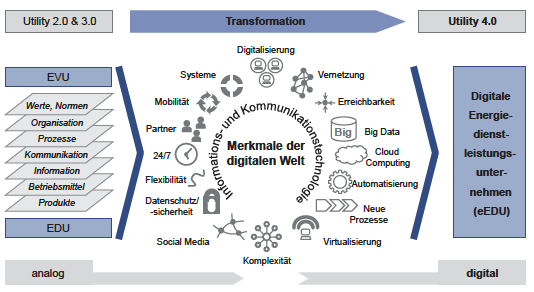
\includegraphics[width=1.0\linewidth]{kalalysator_utility_40.png}
  \caption[Digitale Welt als Katalysator für Utility 4.0 ]{Digitale Welt als Katalysator für Utility 4.0 \citep[S. 17]{Doleski2016}}
\end{figure}
